\chapter{Vectores}

\begin{theorybox}{Trazabilidad del capitulo}
Este capitulo desarrolla las secciones \texttt{C06.S01-C06.S06} de la matriz de cobertura a
partir de \texttt{sources/Relacion ejercicios temas 6 y 7.pdf}. La idea central es usar los
vectores como lenguaje comun para describir posiciones, direcciones, angulos y construcciones
planas en \(\R^2\).
\end{theorybox}

\section{[C06.S01] Bases y dependencia en \texorpdfstring{\(\R^2\)}{R2}}

\subsection*{Objetivos de aprendizaje}
\begin{itemize}
  \item Decidir si dos vectores forman una base de \(\R^2\).
  \item Expresar un vector en una base no canonica.
\end{itemize}

\subsection*{Prerrequisitos}
\begin{itemize}
  \item Resolucion de sistemas lineales \(2\times 2\).
\end{itemize}

\begin{theorybox}{Idea minima}
Dos vectores de \(\R^2\) forman una base si son linealmente independientes. En coordenadas, eso
equivale a que el determinante de la matriz formada por sus componentes sea distinto de cero.
\end{theorybox}

\begin{methodbox}{Como reconocer y resolver}
\begin{enumerate}
  \item Coloca los vectores como columnas de una matriz \(2\times 2\).
  \item Calcula el determinante.
  \item Si el determinante no es cero, forman base y puedes usarla para descomponer otros vectores.
\end{enumerate}
\end{methodbox}

\begin{solvedexample}{[EX-C06.S01-01] Comprobar base y cambiar coordenadas}
Sean
\[
u=(1,2),\qquad v=(3,5),\qquad w=(7,11).
\]
Decide si \(u\) y \(v\) forman una base de \(\R^2\) y expresa \(w\) como combinacion lineal de
\(u\) y \(v\).

\textbf{Desarrollo.} El determinante asociado es
\[
\begin{vmatrix}
1 & 3\\
2 & 5
\end{vmatrix}=1\cdot 5-3\cdot 2=-1\neq 0.
\]
Luego \(u\) y \(v\) forman una base.

Buscamos \(a\) y \(b\) tales que
\[
au+bv=w.
\]
Eso lleva al sistema
\[
\begin{cases}
a+3b=7,\\
2a+5b=11.
\end{cases}
\]
Restando el doble de la primera a la segunda:
\[
-b=-3 \Longrightarrow b=3.
\]
Entonces
\[
a+9=7 \Longrightarrow a=-2.
\]

\textbf{Respuesta final.}
\[
u \text{ y } v \text{ forman una base de } \R^2,
\qquad
w=-2u+3v.
\]
\end{solvedexample}

\begin{commonerror}{Confundir distintos con independientes}
Que dos vectores no sean iguales no basta para que formen base. Si uno es multiplo del otro,
siguen siendo dependientes.
\end{commonerror}

\begin{guidedexercise}{[GX-C06.S01-01] Detectar dependencia}
Decide si \((2,1)\) y \((4,2)\) forman base de \(\R^2\).

\textbf{Pista 1.} Uno es multiplo del otro.
\end{guidedexercise}

\begin{shortanswer}{[GX-C06.S01-01]}
No. Son dependientes y no forman base.
\end{shortanswer}

\begin{fullsolution}{[GX-C06.S01-01]}
Como
\[
(4,2)=2(2,1),
\]
los vectores son dependientes. Por tanto, no forman base.
\end{fullsolution}

\begin{guidedexercise}{[GX-C06.S01-02] Coordenadas en otra base}
Expresa \((3,1)\) en la base formada por \(u=(1,1)\) y \(v=(1,-1)\).

\textbf{Pista 1.} Busca \(a\) y \(b\) con \(au+bv=(3,1)\).
\end{guidedexercise}

\begin{shortanswer}{[GX-C06.S01-02]}
\[
(3,1)=2u+v.
\]
\end{shortanswer}

\begin{fullsolution}{[GX-C06.S01-02]}
El sistema es
\[
\begin{cases}
a+b=3,\\
a-b=1.
\end{cases}
\]
Sumando, \(2a=4\), luego \(a=2\). Despues \(b=1\).
\end{fullsolution}

\subsection*{Practica autonoma graduada}
\begin{exercise}{[PX-C06.S01-01] Decide si \((1,0)\) y \((0,1)\) forman base de \(\R^2\).}
\end{exercise}
\begin{exercise}{[PX-C06.S01-02] Decide si \((1,3)\) y \((2,6)\) forman base de \(\R^2\).}
\end{exercise}
\begin{exercise}{[PX-C06.S01-03] Halla \(k\) para que \((1,2)\) y \((k,6)\) sean dependientes.}
\end{exercise}
\begin{exercise}{[PX-C06.S01-04] Halla el valor de \(a\) para que \((a,1)\) y \((2,3)\) no formen base.}
\end{exercise}
\begin{exercise}{[PX-C06.S01-05] Expresa \((5,1)\) en la base \(u=(1,1)\), \(v=(2,-1)\).}
\end{exercise}
\begin{exercise}{[PX-C06.S01-06] Decide si \((0,1)\) y \((2,0)\) forman base de \(\R^2\).}
\end{exercise}

\begin{shortanswer}{C06.S01 practica autonoma}
\begin{enumerate}[label=\textbf{PX-C06.S01-\arabic*:}, leftmargin=*]
  \item Si
  \item No
  \item \(k=3\)
  \item \(a=\frac{2}{3}\)
  \item \((5,1)=\frac{7}{3}u+\frac{4}{3}v\)
  \item Si
\end{enumerate}
\end{shortanswer}

\begin{fullsolution}{C06.S01 practica autonoma}
\begin{enumerate}[label=\textbf{PX-C06.S01-\arabic*:}, leftmargin=*]
  \item El determinante vale \(1\), luego si forman base.
  \item \((2,6)=2(1,3)\), asi que no forman base.
  \item La dependencia exige \(6=2k\), luego \(k=3\).
  \item El determinante es \(3a-2\). Para que no formen base debe anularse.
  \item Buscando \(a\) y \(b\),
  \[
  \begin{cases}
  a+2b=5,\\
  a-b=1,
  \end{cases}
  \]
  de donde \(b=\frac{4}{3}\) y \(a=\frac{7}{3}\).
  \item El determinante vale \(-2\), distinto de cero.
\end{enumerate}
\end{fullsolution}

\section{[C06.S02] Operaciones con vectores}

\subsection*{Objetivos de aprendizaje}
\begin{itemize}
  \item Sumar, restar y multiplicar vectores por escalares.
  \item Interpretar combinaciones lineales sencillas.
\end{itemize}

\subsection*{Prerrequisitos}
\begin{itemize}
  \item Operaciones con numeros reales.
\end{itemize}

\begin{theorybox}{Idea minima}
Las operaciones se hacen coordenada a coordenada:
\[
(a,b)+(c,d)=(a+c,b+d),
\qquad
\lambda(a,b)=(\lambda a,\lambda b).
\]
Una combinacion lineal mezcla ambas ideas a la vez.
\end{theorybox}

\begin{methodbox}{Como reconocer y resolver}
\begin{enumerate}
  \item Multiplica primero por escalares si aparecen.
  \item Suma o resta despues cada coordenada.
  \item Comprueba el signo de cada componente al final.
\end{enumerate}
\end{methodbox}

\begin{solvedexample}{[EX-C06.S02-01] Dos combinaciones lineales}
Sean
\[
u=(2,-1),\qquad v=(1,3).
\]
Calcula \(2u-v\) y \(3u+2v\).

\textbf{Desarrollo.}
\[
2u-v=(4,-2)-(1,3)=(3,-5).
\]
\[
3u+2v=(6,-3)+(2,6)=(8,3).
\]

\textbf{Respuesta final.}
\[
2u-v=(3,-5),
\qquad
3u+2v=(8,3).
\]
\end{solvedexample}

\begin{commonerror}{Olvidar repartir el signo menos}
Restar un vector significa restar sus dos coordenadas. El error tipico es cambiar solo la
primera y dejar la segunda igual.
\end{commonerror}

\begin{guidedexercise}{[GX-C06.S02-01] Suma directa}
Calcula \((1,2)+(-3,4)\).
\end{guidedexercise}

\begin{shortanswer}{[GX-C06.S02-01]}
\[
(-2,6).
\]
\end{shortanswer}

\begin{fullsolution}{[GX-C06.S02-01]}
\[
(1,2)+(-3,4)=(-2,6).
\]
\end{fullsolution}

\begin{guidedexercise}{[GX-C06.S02-02] Escalar y resta}
Calcula \(2(3,-1)-(1,5)\).
\end{guidedexercise}

\begin{shortanswer}{[GX-C06.S02-02]}
\[
(5,-7).
\]
\end{shortanswer}

\begin{fullsolution}{[GX-C06.S02-02]}
\[
2(3,-1)=(6,-2),
\]
y por tanto
\[
(6,-2)-(1,5)=(5,-7).
\]
\end{fullsolution}

\subsection*{Practica autonoma graduada}
\begin{exercise}{[PX-C06.S02-01] Si \(u=(2,1)\) y \(v=(-1,4)\), calcula \(u+v\).}
\end{exercise}
\begin{exercise}{[PX-C06.S02-02] Si \(u=(5,0)\) y \(v=(2,-3)\), calcula \(u-v\).}
\end{exercise}
\begin{exercise}{[PX-C06.S02-03] Si \(u=(1,-2)\), calcula \(-3u\).}
\end{exercise}
\begin{exercise}{[PX-C06.S02-04] Si \(u=(4,1)\) y \(v=(2,5)\), calcula \(\frac{1}{2}(u+v)\).}
\end{exercise}
\begin{exercise}{[PX-C06.S02-05] Si \(u=(3,-2)\) y \(v=(-1,1)\), calcula \(4u+v\).}
\end{exercise}
\begin{exercise}{[PX-C06.S02-06] Si \(u=(2,3)\) y \(v=(4,-1)\), calcula \(v-2u\).}
\end{exercise}

\begin{shortanswer}{C06.S02 practica autonoma}
\begin{enumerate}[label=\textbf{PX-C06.S02-\arabic*:}, leftmargin=*]
  \item \((1,5)\)
  \item \((3,3)\)
  \item \((-3,6)\)
  \item \((3,3)\)
  \item \((11,-7)\)
  \item \((0,-7)\)
\end{enumerate}
\end{shortanswer}

\begin{fullsolution}{C06.S02 practica autonoma}
\begin{enumerate}[label=\textbf{PX-C06.S02-\arabic*:}, leftmargin=*]
  \item \((2,1)+(-1,4)=(1,5)\).
  \item \((5,0)-(2,-3)=(3,3)\).
  \item \(-3(1,-2)=(-3,6)\).
  \item \(\frac{1}{2}(6,6)=(3,3)\).
  \item \(4(3,-2)+(-1,1)=(12,-8)+(-1,1)=(11,-7)\).
  \item \((4,-1)-(4,6)=(0,-7)\).
\end{enumerate}
\end{fullsolution}

\section{[C06.S03] Modulo, argumento y vectores unitarios}

\subsection*{Objetivos de aprendizaje}
\begin{itemize}
  \item Calcular modulo y argumento de un vector.
  \item Construir vectores unitarios y resolver condiciones de norma.
\end{itemize}

\subsection*{Prerrequisitos}
\begin{itemize}
  \item Pitagoras y trigonometria basica.
\end{itemize}

\begin{theorybox}{Idea minima}
El modulo de \(u=(a,b)\) es
\[
|u|=\sqrt{a^2+b^2}.
\]
Su argumento es el angulo que forma con el eje \(X\) positivo. En este capitulo tomaremos el
argumento principal en \([0,2\pi)\). Un vector unitario tiene modulo \(1\).
\end{theorybox}

\begin{methodbox}{Como reconocer y resolver}
\begin{enumerate}
  \item Usa Pitagoras para hallar el modulo.
  \item Localiza el cuadrante para fijar el argumento.
  \item Si piden un vector unitario, divide por el modulo.
\end{enumerate}
\end{methodbox}

\begin{solvedexample}{[EX-C06.S03-01] Modulo, argumento y unitario}
Sea \(u=(1,\sqrt{3})\). Calcula su modulo, su argumento y el vector unitario de la misma
direccion y sentido.

\textbf{Desarrollo.} El modulo es
\[
|u|=\sqrt{1^2+(\sqrt{3})^2}=\sqrt{4}=2.
\]
Como
\[
\cos \alpha=\frac{1}{2},
\qquad
\sen \alpha=\frac{\sqrt{3}}{2},
\]
se tiene \(\alpha=\frac{\pi}{3}\).

El vector unitario es
\[
\frac{u}{|u|}=\left(\frac{1}{2},\frac{\sqrt{3}}{2}\right).
\]

\textbf{Respuesta final.}
\[
|u|=2,
\qquad
\arg(u)=\frac{\pi}{3},
\qquad
\widehat{u}=\left(\frac{1}{2},\frac{\sqrt{3}}{2}\right).
\]
\end{solvedexample}

\begin{commonerror}{Dar el argumento correcto con cuadrante incorrecto}
El angulo de referencia no basta. Un vector en el segundo o cuarto cuadrante comparte tangente
con otros angulos, asi que hay que mirar los signos de ambas coordenadas.
\end{commonerror}

\begin{guidedexercise}{[GX-C06.S03-01] Segundo cuadrante}
Calcula el modulo y el argumento de \(v=(-1,1)\).

\textbf{Pista 1.} El modulo es \(\sqrt{2}\) y el angulo de referencia es \(45^\circ\).
\end{guidedexercise}

\begin{shortanswer}{[GX-C06.S03-01]}
\[
|v|=\sqrt{2},
\qquad
\arg(v)=\frac{3\pi}{4}.
\]
\end{shortanswer}

\begin{fullsolution}{[GX-C06.S03-01]}
\[
|v|=\sqrt{(-1)^2+1^2}=\sqrt{2}.
\]
El vector esta en el segundo cuadrante y su angulo de referencia es \(\frac{\pi}{4}\), luego
\[
\arg(v)=\pi-\frac{\pi}{4}=\frac{3\pi}{4}.
\]
\end{fullsolution}

\begin{guidedexercise}{[GX-C06.S03-02] Condicion de modulo}
Halla \(a>0\) si el vector \((a,4)\) tiene modulo \(5\).

\textbf{Pista 1.} Plantea \(a^2+4^2=5^2\).
\end{guidedexercise}

\begin{shortanswer}{[GX-C06.S03-02]}
\[
a=3.
\]
\end{shortanswer}

\begin{fullsolution}{[GX-C06.S03-02]}
\[
a^2+16=25 \Longrightarrow a^2=9.
\]
Como \(a>0\), se sigue que \(a=3\).
\end{fullsolution}

\subsection*{Practica autonoma graduada}
\begin{exercise}{[PX-C06.S03-01] Halla el modulo de \((3,4)\).}
\end{exercise}
\begin{exercise}{[PX-C06.S03-02] Halla el argumento principal de \((0,-2)\).}
\end{exercise}
\begin{exercise}{[PX-C06.S03-03] Halla un vector unitario con la misma direccion y sentido que \((0,5)\).}
\end{exercise}
\begin{exercise}{[PX-C06.S03-04] Halla \(k>0\) si el vector \((k,4)\) tiene modulo \(5\).}
\end{exercise}
\begin{exercise}{[PX-C06.S03-05] Halla un vector de modulo \(2\) y argumento \(150^\circ\).}
\end{exercise}
\begin{exercise}{[PX-C06.S03-06] Halla el modulo y el argumento principal de \((-\sqrt{3},1)\).}
\end{exercise}

\begin{shortanswer}{C06.S03 practica autonoma}
\begin{enumerate}[label=\textbf{PX-C06.S03-\arabic*:}, leftmargin=*]
  \item \(5\)
  \item \(\frac{3\pi}{2}\)
  \item \((0,1)\)
  \item \(k=3\)
  \item \((-\sqrt{3},1)\)
  \item Modulo \(2\), argumento \(\frac{5\pi}{6}\)
\end{enumerate}
\end{shortanswer}

\begin{fullsolution}{C06.S03 practica autonoma}
\begin{enumerate}[label=\textbf{PX-C06.S03-\arabic*:}, leftmargin=*]
  \item \(\sqrt{3^2+4^2}=5\).
  \item El vector cae sobre el eje \(Y\) negativo.
  \item \((0,5)\) dividido entre su modulo \(5\) da \((0,1)\).
  \item Es el mismo calculo que en el guiado.
  \item
  \[
  2(\cos 150^\circ,\sen 150^\circ)=2\left(-\frac{\sqrt{3}}{2},\frac{1}{2}\right)=(-\sqrt{3},1).
  \]
  \item
  \[
  |u|=\sqrt{3+1}=2,
  \]
  y el vector esta en el segundo cuadrante con referencia \(\frac{\pi}{6}\).
\end{enumerate}
\end{fullsolution}

\section{[C06.S04] Producto escalar y angulo entre vectores}

\subsection*{Objetivos de aprendizaje}
\begin{itemize}
  \item Calcular productos escalares.
  \item Deducir perpendicularidad, modulos y angulos.
\end{itemize}

\subsection*{Prerrequisitos}
\begin{itemize}
  \item Modulo de un vector y trigonometria basica.
\end{itemize}

\begin{theorybox}{Idea minima}
Para \(u=(a,b)\) y \(v=(c,d)\),
\[
u\cdot v=ac+bd.
\]
Ademas,
\[
u\cdot v=|u|\,|v|\,\cos \theta,
\]
donde \(\theta\) es el angulo entre ambos vectores. Si \(u\cdot v=0\), los vectores son
perpendiculares.
\end{theorybox}

\begin{methodbox}{Como reconocer y resolver}
\begin{enumerate}
  \item Calcula primero \(u\cdot v\).
  \item Si piden el angulo, calcula tambien los modulos.
  \item Usa la formula con \(\cos \theta\) o la condicion de perpendicularidad.
\end{enumerate}
\end{methodbox}

\begin{solvedexample}{[EX-C06.S04-01] Perpendicularidad por producto escalar}
Sean \(u=(1,2)\) y \(v=(2,-1)\). Calcula \(u\cdot v\) y el angulo entre ambos.

\textbf{Desarrollo.}
\[
u\cdot v=1\cdot 2+2\cdot (-1)=0.
\]
Si el producto escalar vale \(0\), entonces los vectores son perpendiculares, asi que el angulo
entre ellos es
\[
\theta=\frac{\pi}{2}.
\]

\textbf{Respuesta final.}
\[
u\cdot v=0,
\qquad
\theta=\frac{\pi}{2}.
\]
\end{solvedexample}

\begin{commonerror}{Olvidar multiplicar coordenadas correspondientes}
El producto escalar no es sumar todas las coordenadas. Hay que multiplicar primera con primera
y segunda con segunda antes de sumar.
\end{commonerror}

\begin{guidedexercise}{[GX-C06.S04-01] Angulo con el eje \(X\)}
Halla el angulo entre \((1,0)\) y \((1,1)\).

\textbf{Pista 1.} El primer vector es unitario y apunta sobre el eje \(X\).
\end{guidedexercise}

\begin{shortanswer}{[GX-C06.S04-01]}
\[
\theta=\frac{\pi}{4}.
\]
\end{shortanswer}

\begin{fullsolution}{[GX-C06.S04-01]}
\[
(1,0)\cdot (1,1)=1,
\qquad
|(1,0)|=1,
\qquad
|(1,1)|=\sqrt{2}.
\]
Entonces
\[
\cos \theta=\frac{1}{\sqrt{2}}=\frac{\sqrt{2}}{2},
\]
y por tanto \(\theta=\frac{\pi}{4}\).
\end{fullsolution}

\begin{guidedexercise}{[GX-C06.S04-02] Vector paralelo con modulo fijado}
Halla un vector de modulo \(4\) con la misma direccion y sentido que \((3,4)\).

\textbf{Pista 1.} Primero normaliza \((3,4)\).
\end{guidedexercise}

\begin{shortanswer}{[GX-C06.S04-02]}
\[
\left(\frac{12}{5},\frac{16}{5}\right).
\]
\end{shortanswer}

\begin{fullsolution}{[GX-C06.S04-02]}
Como \(|(3,4)|=5\), el unitario asociado es \(\left(\frac{3}{5},\frac{4}{5}\right)\). Al
multiplicar por \(4\), se obtiene
\[
\left(\frac{12}{5},\frac{16}{5}\right).
\]
\end{fullsolution}

\subsection*{Practica autonoma graduada}
\begin{exercise}{[PX-C06.S04-01] Calcula \((2,3)\cdot (1,-1)\).}
\end{exercise}
\begin{exercise}{[PX-C06.S04-02] Decide si \((1,2)\) y \((2,-1)\) son perpendiculares.}
\end{exercise}
\begin{exercise}{[PX-C06.S04-03] Halla el angulo entre \((1,1)\) y \((1,-1)\).}
\end{exercise}
\begin{exercise}{[PX-C06.S04-04] Halla el angulo entre \((1,0)\) y \((1,\sqrt{3})\).}
\end{exercise}
\begin{exercise}{[PX-C06.S04-05] Halla un vector de modulo \(5\), en el primer cuadrante, que forme \(60^\circ\) con el eje \(X\).}
\end{exercise}
\begin{exercise}{[PX-C06.S04-06] Si \(|u|=3\), \(|v|=4\) y el angulo entre ellos es \(60^\circ\), calcula \(u\cdot v\).}
\end{exercise}

\begin{shortanswer}{C06.S04 practica autonoma}
\begin{enumerate}[label=\textbf{PX-C06.S04-\arabic*:}, leftmargin=*]
  \item \(-1\)
  \item Si
  \item \(\frac{\pi}{2}\)
  \item \(\frac{\pi}{3}\)
  \item \(\left(\frac{5}{2},\frac{5\sqrt{3}}{2}\right)\)
  \item \(6\)
\end{enumerate}
\end{shortanswer}

\begin{fullsolution}{C06.S04 practica autonoma}
\begin{enumerate}[label=\textbf{PX-C06.S04-\arabic*:}, leftmargin=*]
  \item \(2\cdot 1+3\cdot (-1)=-1\).
  \item El producto escalar es \(0\), luego si.
  \item El producto escalar vale \(0\), asi que el angulo es recto.
  \item
  \[
  \cos \theta=\frac{1}{|(1,\sqrt{3})|}=\frac{1}{2},
  \]
  y por tanto \(\theta=\frac{\pi}{3}\).
  \item
  \[
  5(\cos 60^\circ,\sen 60^\circ)=\left(\frac{5}{2},\frac{5\sqrt{3}}{2}\right).
  \]
  \item
  \[
  u\cdot v=|u|\,|v|\,\cos 60^\circ=3\cdot 4\cdot \frac{1}{2}=6.
  \]
\end{enumerate}
\end{fullsolution}

\section{[C06.S05] Paralelismo, perpendicularidad y alineacion}

\subsection*{Objetivos de aprendizaje}
\begin{itemize}
  \item Decidir si dos vectores son paralelos o perpendiculares.
  \item Comprobar si tres puntos estan alineados.
\end{itemize}

\subsection*{Prerrequisitos}
\begin{itemize}
  \item Producto escalar y proporcionalidad entre vectores.
\end{itemize}

\begin{theorybox}{Idea minima}
Dos vectores son paralelos si uno es multiplo del otro. Son perpendiculares si su producto
escalar vale cero. Tres puntos \(A\), \(B\) y \(C\) estan alineados si \(\overrightarrow{AB}\) y
\(\overrightarrow{AC}\) son paralelos.
\end{theorybox}

\begin{methodbox}{Como reconocer y resolver}
\begin{enumerate}
  \item Para paralelismo, compara razones entre coordenadas.
  \item Para perpendicularidad, calcula el producto escalar.
  \item Para alineacion, construye dos vectores con origen comun.
\end{enumerate}
\end{methodbox}

\begin{solvedexample}{[EX-C06.S05-01] Relacion entre vectores y puntos}
Estudia la relacion entre \(u=(2,1)\) y \(v=(6,3)\). Despues, decide si
\[
A(0,0),\quad B(2,1),\quad C(4,2)
\]
estan alineados.

\textbf{Desarrollo.} Como
\[
v=3u,
\]
los vectores son paralelos.

Por otra parte,
\[
\overrightarrow{AB}=(2,1),
\qquad
\overrightarrow{AC}=(4,2)=2(2,1).
\]
Como \(\overrightarrow{AB}\) y \(\overrightarrow{AC}\) son paralelos, los tres puntos estan
alineados.

\textbf{Respuesta final.}
\[
u \parallel v,
\qquad
A,\ B,\ C \text{ estan alineados}.
\]
\end{solvedexample}

\begin{commonerror}{Comparar solo una coordenada}
Que la primera coordenada sea proporcional no basta. El paralelismo exige la misma razon en las
dos coordenadas.
\end{commonerror}

\begin{guidedexercise}{[GX-C06.S05-01] Perpendicularidad}
Decide si \((1,-2)\) y \((2,1)\) son perpendiculares.

\textbf{Pista 1.} Calcula su producto escalar.
\end{guidedexercise}

\begin{shortanswer}{[GX-C06.S05-01]}
Si. Son perpendiculares.
\end{shortanswer}

\begin{fullsolution}{[GX-C06.S05-01]}
\[
(1,-2)\cdot (2,1)=2-2=0.
\]
Luego son perpendiculares.
\end{fullsolution}

\begin{guidedexercise}{[GX-C06.S05-02] Alineacion}
Decide si \(A(1,0)\), \(B(2,2)\) y \(C(3,4)\) estan alineados.

\textbf{Pista 1.} Compara \(\overrightarrow{AB}\) y \(\overrightarrow{AC}\).
\end{guidedexercise}

\begin{shortanswer}{[GX-C06.S05-02]}
Si. Estan alineados.
\end{shortanswer}

\begin{fullsolution}{[GX-C06.S05-02]}
\[
\overrightarrow{AB}=(1,2),
\qquad
\overrightarrow{AC}=(2,4)=2(1,2).
\]
Por tanto, los tres puntos estan alineados.
\end{fullsolution}

\subsection*{Practica autonoma graduada}
\begin{exercise}{[PX-C06.S05-01] Decide la relacion entre \((3,2)\) y \((6,4)\).}
\end{exercise}
\begin{exercise}{[PX-C06.S05-02] Decide la relacion entre \((1,3)\) y \((3,-1)\).}
\end{exercise}
\begin{exercise}{[PX-C06.S05-03] Decide si \(A(0,1)\), \(B(2,3)\) y \(C(4,5)\) estan alineados.}
\end{exercise}
\begin{exercise}{[PX-C06.S05-04] Decide si \(A(1,1)\), \(B(2,4)\) y \(C(4,5)\) estan alineados.}
\end{exercise}
\begin{exercise}{[PX-C06.S05-05] Halla \(k\) para que \((k,2)\) sea perpendicular a \((1,-4)\).}
\end{exercise}
\begin{exercise}{[PX-C06.S05-06] Halla \(k\) para que \((2,k)\) sea paralelo a \((6,9)\).}
\end{exercise}

\begin{shortanswer}{C06.S05 practica autonoma}
\begin{enumerate}[label=\textbf{PX-C06.S05-\arabic*:}, leftmargin=*]
  \item Paralelos
  \item Perpendiculares
  \item Si
  \item No
  \item \(k=8\)
  \item \(k=3\)
\end{enumerate}
\end{shortanswer}

\begin{fullsolution}{C06.S05 practica autonoma}
\begin{enumerate}[label=\textbf{PX-C06.S05-\arabic*:}, leftmargin=*]
  \item \((6,4)=2(3,2)\), luego son paralelos.
  \item \(1\cdot 3+3\cdot (-1)=0\), luego son perpendiculares.
  \item \(\overrightarrow{AB}=(2,2)\) y \(\overrightarrow{AC}=(4,4)\), luego si.
  \item \(\overrightarrow{AB}=(1,3)\) y \(\overrightarrow{AC}=(3,4)\) no son paralelos.
  \item \(k\cdot 1+2\cdot (-4)=0\), de donde \(k=8\).
  \item La razon de proporcionalidad es \(3\), asi que \(k=3\).
\end{enumerate}
\end{fullsolution}

\section{[C06.S06] Construcciones con vectores y paralelogramos}

\subsection*{Objetivos de aprendizaje}
\begin{itemize}
  \item Hallar puntos a partir de relaciones vectoriales.
  \item Completar paralelogramos y usar puntos medios.
\end{itemize}

\subsection*{Prerrequisitos}
\begin{itemize}
  \item Operaciones con vectores y coordenadas de puntos.
\end{itemize}

\begin{theorybox}{Idea minima}
En un paralelogramo \(ABCD\),
\[
\overrightarrow{AB}=\overrightarrow{DC},
\qquad
\overrightarrow{AD}=\overrightarrow{BC},
\qquad
C=B+D-A.
\]
Los puntos medios y traslaciones tambien se describen con sumas y restas de vectores.

\begin{center}
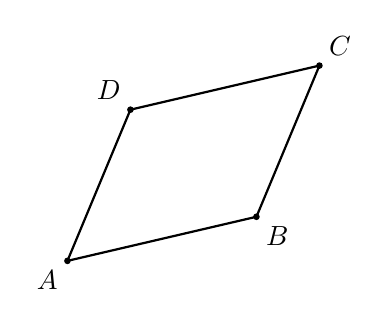
\begin{tikzpicture}[scale=0.8]
  \coordinate (A) at (0,0);
  \coordinate (B) at (3,0.7);
  \coordinate (D) at (1,2.4);
  \coordinate (C) at (4,3.1);
  \draw[thick] (A) -- (B) -- (C) -- (D) -- cycle;
  \fill (A) circle (1.5pt) node[below left] {\(A\)};
  \fill (B) circle (1.5pt) node[below right] {\(B\)};
  \fill (C) circle (1.5pt) node[above right] {\(C\)};
  \fill (D) circle (1.5pt) node[above left] {\(D\)};
\end{tikzpicture}
\end{center}
\end{theorybox}

\begin{methodbox}{Como reconocer y resolver}
\begin{enumerate}
  \item Traduce el dato geometrico a una igualdad de vectores.
  \item Escribe las coordenadas de cada vector como resta de puntos.
  \item Despeja el punto desconocido al final.
\end{enumerate}
\end{methodbox}

\begin{solvedexample}{[EX-C06.S06-01] Completar un paralelogramo}
Sean
\[
A(1,1),\qquad B(4,2),\qquad D(2,5).
\]
Halla el cuarto vertice \(C\) del paralelogramo \(ABCD\).

\textbf{Desarrollo.} En un paralelogramo se cumple
\[
\overrightarrow{DC}=\overrightarrow{AB}.
\]
Como
\[
\overrightarrow{AB}=(4-1,2-1)=(3,1),
\]
sumamos ese vector a \(D\):
\[
C=D+\overrightarrow{AB}=(2,5)+(3,1)=(5,6).
\]

\textbf{Respuesta final.}
\[
C(5,6).
\]
\end{solvedexample}

\begin{commonerror}{Restar los puntos en orden incorrecto}
No es lo mismo \(\overrightarrow{AB}=B-A\) que \(A-B\). Cambiar el orden invierte la
direccion y desplaza mal el punto buscado.
\end{commonerror}

\begin{guidedexercise}{[GX-C06.S06-01] Vector entre dos puntos}
Si \(\overrightarrow{AB}=(3,-1)\) y \(\overrightarrow{AC}=(5,2)\), calcula
\(\overrightarrow{BC}\).

\textbf{Pista 1.} Usa \(\overrightarrow{BC}=\overrightarrow{AC}-\overrightarrow{AB}\).
\end{guidedexercise}

\begin{shortanswer}{[GX-C06.S06-01]}
\[
\overrightarrow{BC}=(2,3).
\]
\end{shortanswer}

\begin{fullsolution}{[GX-C06.S06-01]}
\[
\overrightarrow{BC}=(5,2)-(3,-1)=(2,3).
\]
\end{fullsolution}

\begin{guidedexercise}{[GX-C06.S06-02] Punto medio}
Halla el punto medio del segmento con extremos \(A(-1,2)\) y \(B(5,4)\).

\textbf{Pista 1.} Haz la media coordenada a coordenada.
\end{guidedexercise}

\begin{shortanswer}{[GX-C06.S06-02]}
\[
M(2,3).
\]
\end{shortanswer}

\begin{fullsolution}{[GX-C06.S06-02]}
\[
M\left(\frac{-1+5}{2},\frac{2+4}{2}\right)=(2,3).
\]
\end{fullsolution}

\subsection*{Practica autonoma graduada}
\begin{exercise}{[PX-C06.S06-01] Halla el cuarto vertice del paralelogramo con \(A(0,0)\), \(B(3,1)\) y \(D(1,4)\).}
\end{exercise}
\begin{exercise}{[PX-C06.S06-02] Traslada el punto \(P(2,-1)\) con el vector \((-3,4)\).}
\end{exercise}
\begin{exercise}{[PX-C06.S06-03] Halla el punto medio del segmento con extremos \(A(1,5)\) y \(B(7,-1)\).}
\end{exercise}
\begin{exercise}{[PX-C06.S06-04] Si \(M(3,2)\) es el punto medio de \(A(1,0)\) y \(B\), halla \(B\).}
\end{exercise}
\begin{exercise}{[PX-C06.S06-05] Si \(A(1,-1)\) y \(\overrightarrow{AB}=(2,5)\), halla \(B\).}
\end{exercise}
\begin{exercise}{[PX-C06.S06-06] En el paralelogramo \(ABCD\), se conocen \(A(2,1)\), \(B(5,3)\) y \(C(7,6)\). Halla \(D\).}
\end{exercise}

\begin{shortanswer}{C06.S06 practica autonoma}
\begin{enumerate}[label=\textbf{PX-C06.S06-\arabic*:}, leftmargin=*]
  \item \(C(4,5)\)
  \item \(P'(-1,3)\)
  \item \(M(4,2)\)
  \item \(B(5,4)\)
  \item \(B(3,4)\)
  \item \(D(4,4)\)
\end{enumerate}
\end{shortanswer}

\begin{fullsolution}{C06.S06 practica autonoma}
\begin{enumerate}[label=\textbf{PX-C06.S06-\arabic*:}, leftmargin=*]
  \item \(C=B+D-A=(3,1)+(1,4)=(4,5)\).
  \item \(P'=P+(-3,4)=(-1,3)\).
  \item
  \[
  M\left(\frac{1+7}{2},\frac{5+(-1)}{2}\right)=(4,2).
  \]
  \item De la formula del punto medio:
  \[
  \frac{1+x_B}{2}=3,\qquad \frac{0+y_B}{2}=2.
  \]
  \item \(B=A+\overrightarrow{AB}=(1,-1)+(2,5)=(3,4)\).
  \item En un paralelogramo,
  \[
  D=A+C-B=(2,1)+(7,6)-(5,3)=(4,4).
  \]
\end{enumerate}
\end{fullsolution}

\begin{selfcheck}
\begin{itemize}
  \item Distingo cuando necesito un determinante, un producto escalar o una combinacion lineal.
  \item Al trabajar con puntos, traduzco primero a vectores para no mezclar operaciones.
  \item Cuando me piden direccion o sentido, reviso si el vector debe ser unitario.
\end{itemize}
\end{selfcheck}

\begin{extension}{Lenguaje vectorial}
Muchos problemas geometricos que parecen distintos se reducen a la misma idea: comparar
direcciones, longitudes y desplazamientos mediante vectores. Ese cambio de lenguaje simplifica
mucho los calculos posteriores de rectas y distancias.
\end{extension}
